% -----------------------------------------------------------------
% Document class: Article
\documentclass[ a4paper, twoside, 11pt]{article}
\usepackage{../../../macros-general}
\usepackage{../../../macros-article}
% Number of the handout, quiz, exam, etc.
\newcommand{\numero}{02}
\setcounter{numero}{\numero}

% -----------------------------------------------------------------
\begin{document}
\allowdisplaybreaks

\begin{center}
\Large Mec\'anica Vectorial (MECG-1001): Trabajo Aut\'onomo \numero \\[2ex]
\small \textbf{Semestre:} 2017-2018 T\'ermino II \qquad
\textbf{Instructor:} Luis I. Reyes Castro \qquad
\textbf{Paralelo:} 09
\end{center}
\fullskip

% =============================================
\begin{problem}
\textbf{[3 Puntos]} Para el siguiente soporte encuentre la tensi\'on en la cuerda y la reacci\'on en $C$. 

\begin{figure}[htb]
\centering
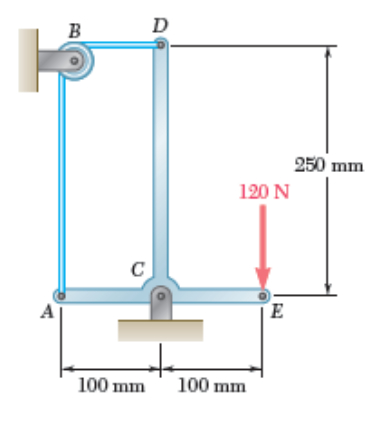
\includegraphics[width=0.4\textwidth]{problema-1.jpg}
\end{figure}

\end{problem}
\vspace{\baselineskip}

% =============================================
\begin{problem}
\textbf{[5 Puntos]} La tuber\'ia soporta las cargas verticales mostradas. Escriba un conjunto de ecuaciones linealmente independientes del cual se pueda encontrar la reacci\'on en $A$ \linebreak y la tensi\'on en cada una de las cuerdas. No resuelva las ecuacioens. 

\begin{figure}[htb]
\centering
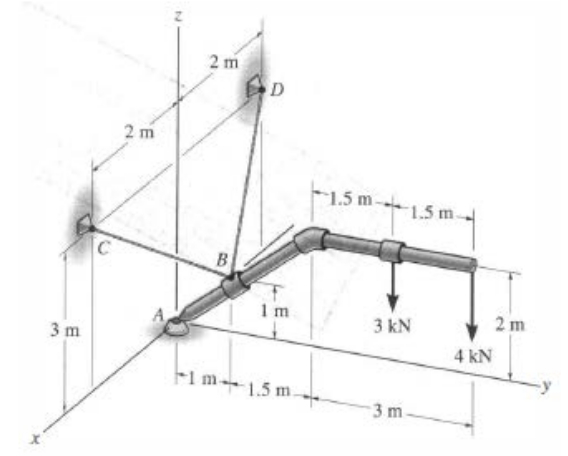
\includegraphics[width=0.5\textwidth]{problema-2.jpg}
\end{figure}

\end{problem}
\vspace{\baselineskip}

\end{document}